\section{Artefact Development Report - T1 2022 (draft)}
\almarginpar{We need some introduction to the section 4 explaining its purpose and its}
\almarginpar{Be clear from above design discussion what the artefact development was to achieve and what part of it the minimum artefact satisfies}
\begin{todolist}
    \item[\done] Discussion on artefact developed (so far) and evaluation of the artefact (if any);
    \item[\done] Details of data collected, experimental procedure;
    \item Lessons learned in the sprint (?);
    \item[\done] Results of the artefact analysis;
\end{todolist}

Notes from Prof.

\begin{todolist}
    \item[\done] How gradient variance is being calculated (formula)
    \item[\done] How do we know that high variance does not simply mean that your gradient function is not just noise (for future works)?
    \item Does it converge eventually (for future works)?
    \item Can you verify that the gradient descent results in a solution (for future works)?
\end{todolist}

\subsection{Development Process}
The minimum viable artefact is a Python notebook file containing Python scripts to run the experiment.
We run the notebook with IBM Quantum Experience, as they provide online services for simulating quantum hardware.
The following sections describe our experiment process.

\subsubsection{The Quantum Emulator}
For this experiment, we are using the Quantum Emulator provided by Qiskit.
The QASM simulator is used to mimic an IBMQ device.
We don't configure the noise model for emulator. 
Additionally, QASM simulator by default has no noise, so we can expect the result to be noise-free.

\subsubsection{Creating Ansatzes}
We have chosen two ansatzes \textit{NLocal} and \textit{TwoLocal} from the Qiskit circuit library due to their wide usage in quantum machine learning.
As discussed in the Research Design section, we configure the ansatz objects such that their gradient variances decrease exponentially with the number of qubits.
These characteristics are:
\begin{itemize}
    \item The circuit depth;
    \item The number of qubits to be measured for the cost function;
    \item The randomised parameters.
\end{itemize}
An example of circuits generated by Qiskit is visualised in Figure \ref{Ansatz samples}.

\todo{maybe show the same qubit with different layers, how to calculate the depth of circuit}
\begin{figure}
    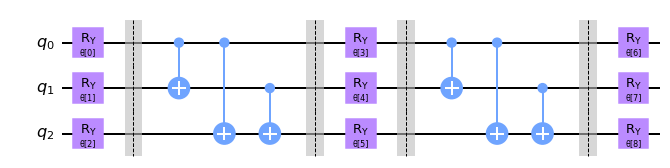
\includegraphics[width=\textwidth]{Artefact/Appendices/ansatz3-2.png}
    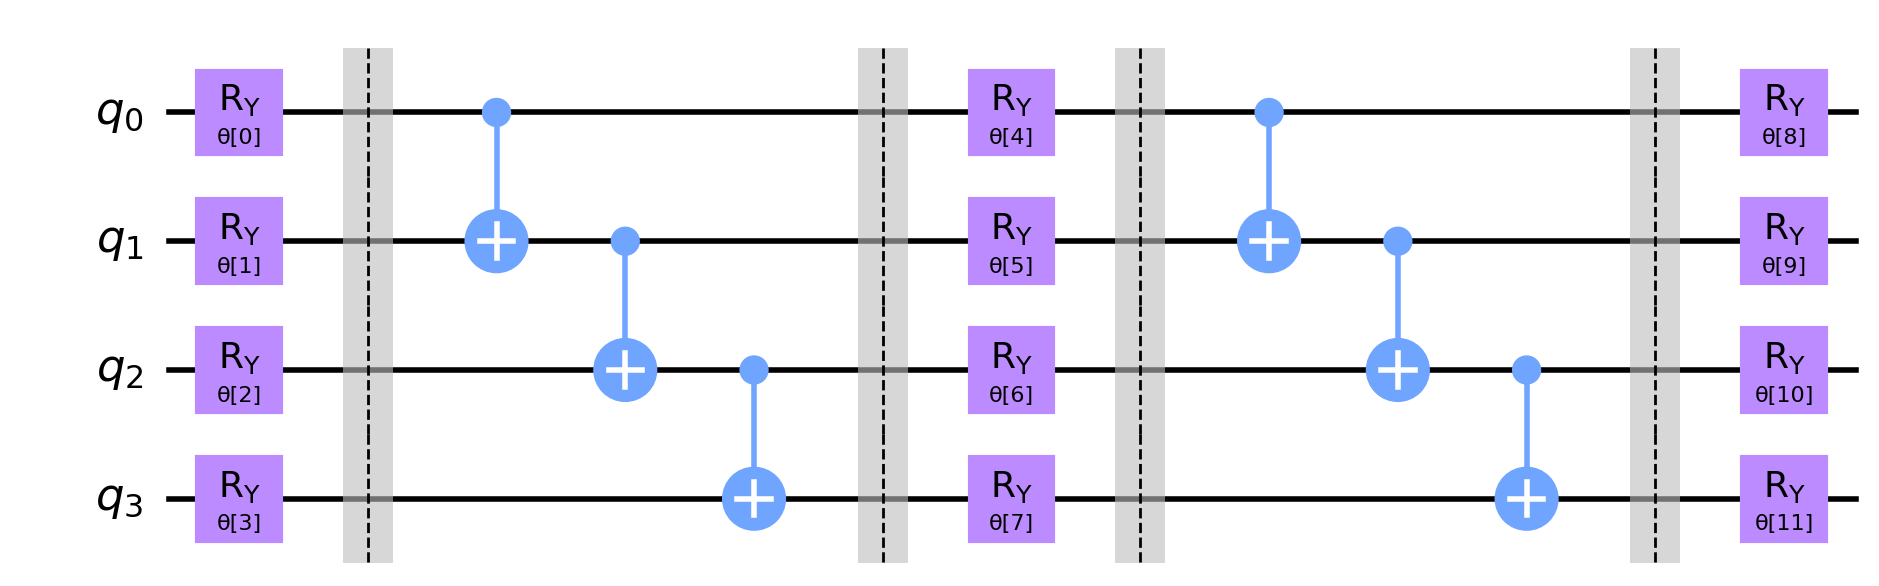
\includegraphics[width=\textwidth]{Artefact/Appendices/ansatz4-2.png}
    \caption{
        Samples of parameterised circuits generated by the Qiskit framework.
        The ansatz is a sequence of rotation layers and entanglement layers.
        Above: an ansatz of three qubits and two repetition layers.
        Below: an ansatz of four qubits and two repetition layers.
    }
    \label{Ansatz samples}
\end{figure}

\subsubsection{Visualise the Gradient}
To calculate the gradient variance, we use the parameter shift rule from Eq. \ref{Parameter-shift rules} as implemented in Qiskit Gradient Framework.
The BP phenomena can be verified when the gradient variance with an increased number of qubits and repetition layers.

To visualise the gradient variances, we have plotted a range of random parameters for each ansatz as the initial starting point.
Such randomised parameters are generated 100 times uniformly to calculate the gradients.
We then plot the variance values of the gradients for different numbers of qubits and repetition values for a range of 2 to 9 qubits and repetition.

In short, we use 100 uniformly randomised parameters to scan the gradient, then we calculate the "slope" of the gradient.

\subsubsection{Experiment with Local Cost Function and Shallow Depth}
The two ansatzes are configured such that their depths are fixed, along with a local cost function.
The \textit{Global Cost Function} is the combined output of all qubits. 
On the other hand, the \textit{Local Cost Function} only compares the values of individual qubits or a subset of qubits \cite{cerezoCostFunctionDependent2021}.

\todo{add: in this case we are using the local cost function like this (describe) and the global like that (describe)}

\subsection{Results and Analysis} \label{Result section}

\subsubsection{Sampling Gradients results}
\begin{table*}
    \centering
    \begin{tabular}{|| l l l ||}
        \hline
        \textbf{Ansatz} & \textbf{Method}                         & \textbf{Variance exponential fit} \\[0.5ex]
        \hline \hline
        Real Amplitude  & \#0: No restriction                     & -0.63                             \\
        Real Amplitude  & \#1: Local Cost function, shallow depth & -0.06                             \\
        Real Amplitude  & \#2: Layerwise Learning                 & -0.57                             \\
        Customised      & \#3: Identity Blocks                    & -0.60                             \\
        \hline
    \end{tabular}
    \caption{
        The phase one of the experiments that we implemented in the Python Notebook.
        We test the same ansatzes with different methods, we record the results as the vanishing rate of gradient when the number of qubits increased.
        The differences between the \emph{fit} values are small.
        However, consider the unit measure is \emph{exponential} (i.e. $10^{-1}, 10^{-2}$) the growth or decay rates can be significant.
    }
    \label{Tab: Experiment Phase 1 Res}
\end{table*}

Table \ref{Tab: Experiment Phase 1 Res} states all the combinations of ansatzes and methods.

The ansatz gradient variances decay as expected for the unrestricted setting.
The decay rate is exponentially fitted with the rate of -0.63.
The figure \ref{Plot ansatzes variance}a shows the results of the ansatz in this configuration.
The semi-log plots portray the variances of gradient from the ansatz in the unrestricted configuration.
Consider that the unit measure for variance is in \emph{exponential} form, so the linear graph is exponentially closer to zero for each qubit added to the circuit.
This result indicates that the cost function landscape becomes flatter and flatter.
Eventually, the gradient would reach a near-zero value across a large plateau, which would be inefficient for any gradient-based optimization algorithm to train the model.
We discussed this phenomenon in Section \ref{Barren Plateaus section}.

\todo{changing the number to actual name}
\begin{figure}
    \centering
    \begin{subfigure}[b]{.49\linewidth}
        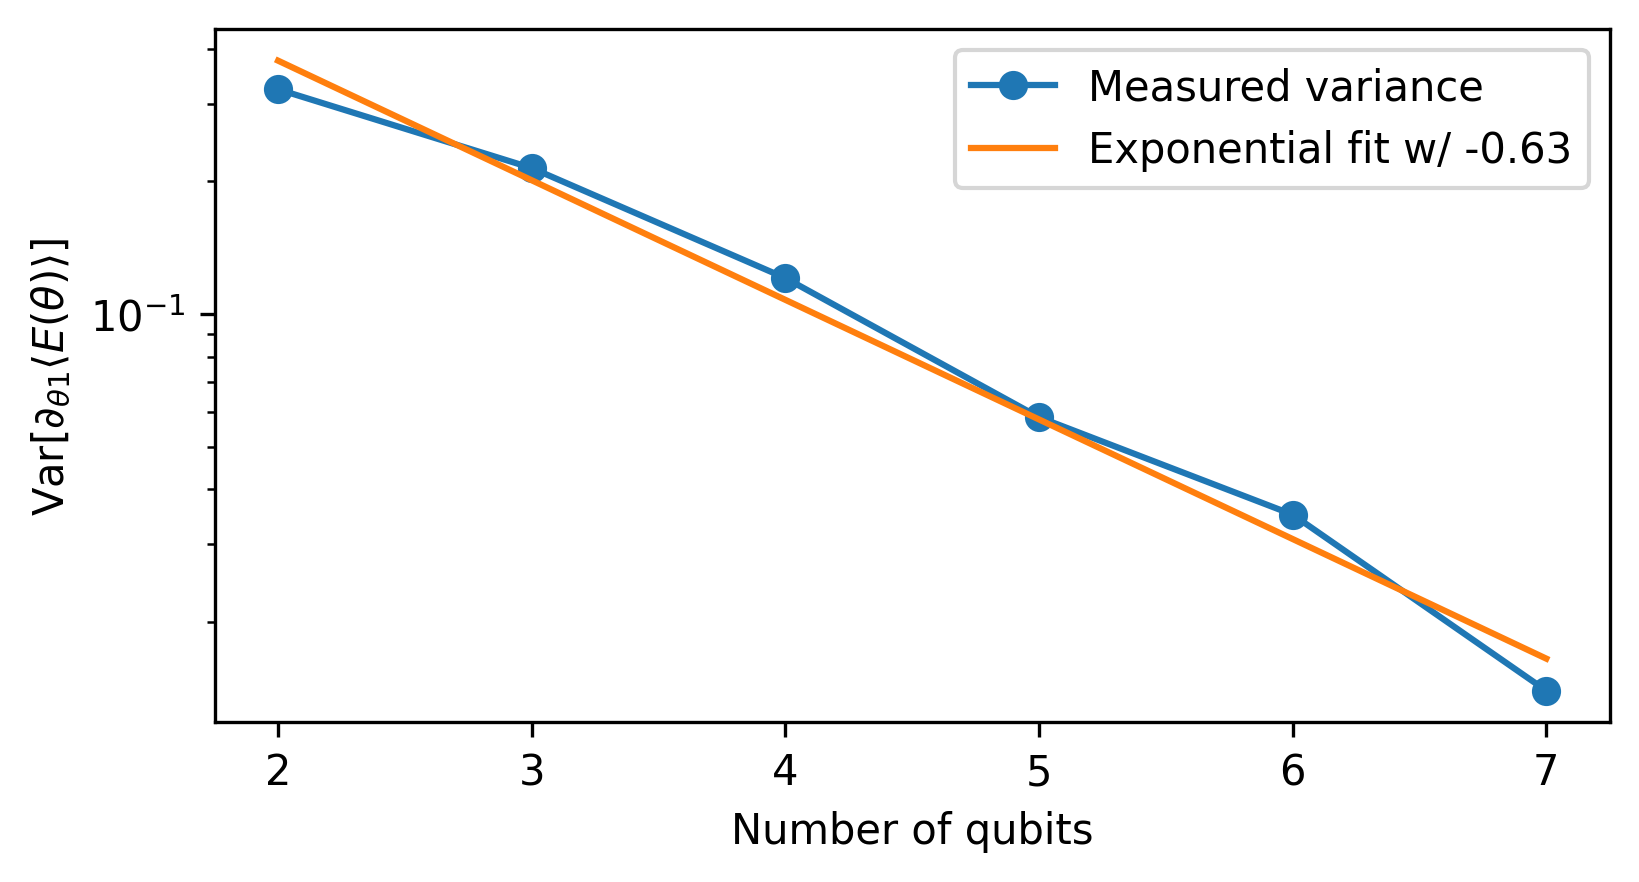
\includegraphics[width=\linewidth]{Artefact/Appendices/var0.png}
        \centerline{0) Default method}
    \end{subfigure}
    \hfill
    \begin{subfigure}[b]{.49\linewidth}
        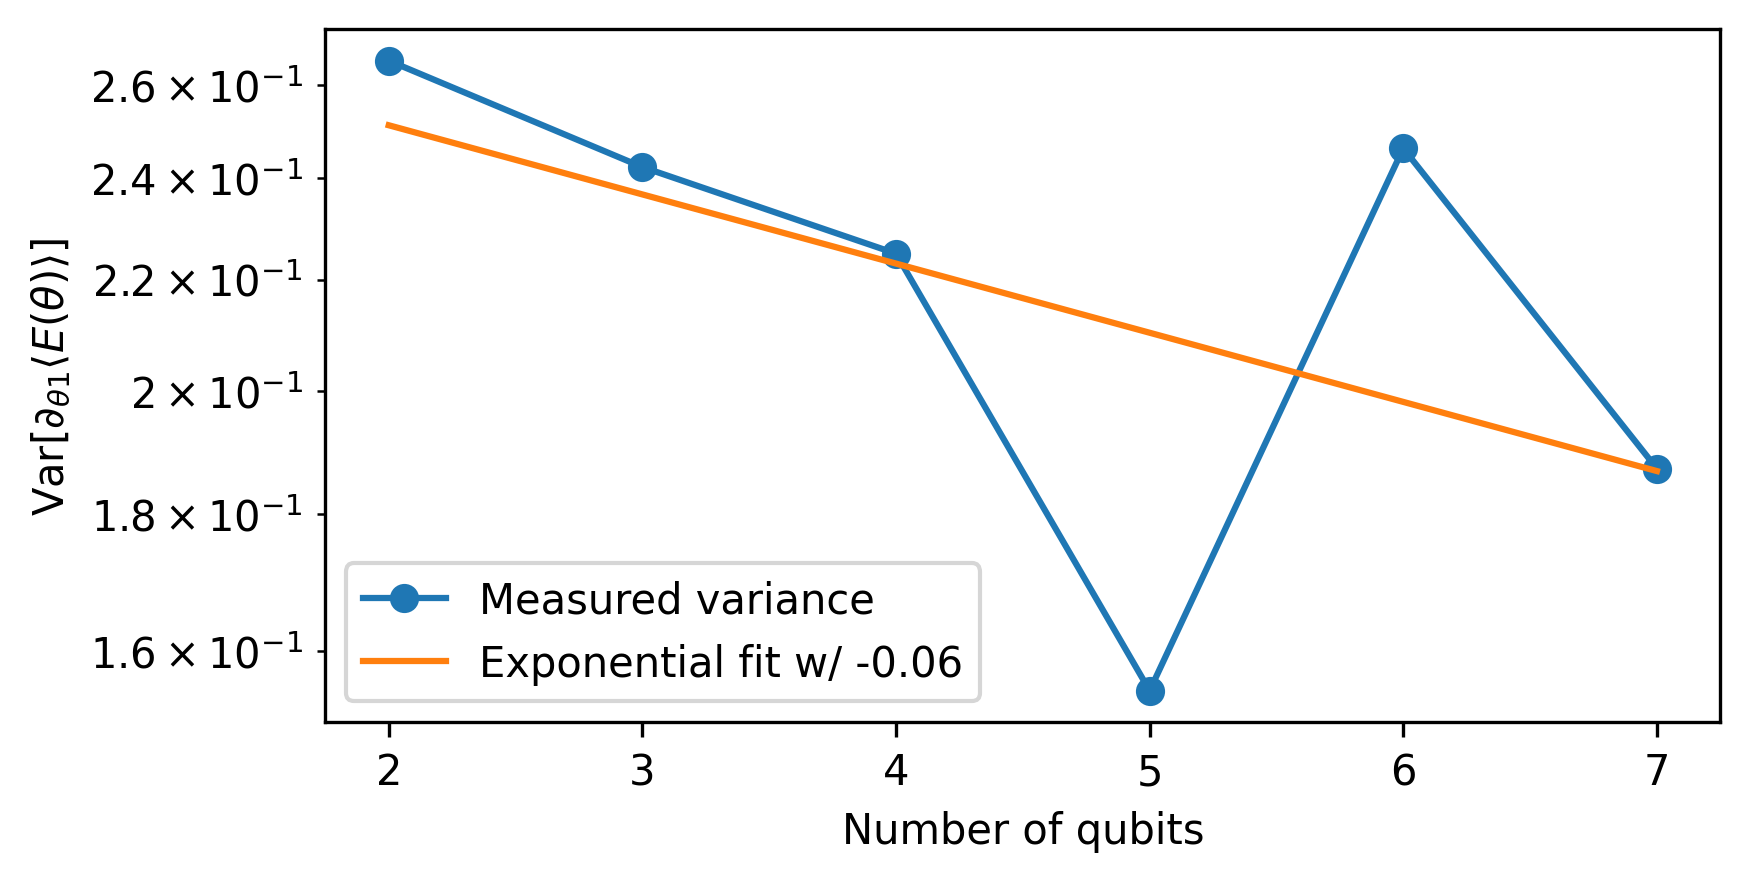
\includegraphics[width=\linewidth]{Artefact/Appendices/var1.png}
        \centerline{1) Shallow circuit and local cost function}
    \end{subfigure}

    \begin{subfigure}[b]{.49\linewidth}
        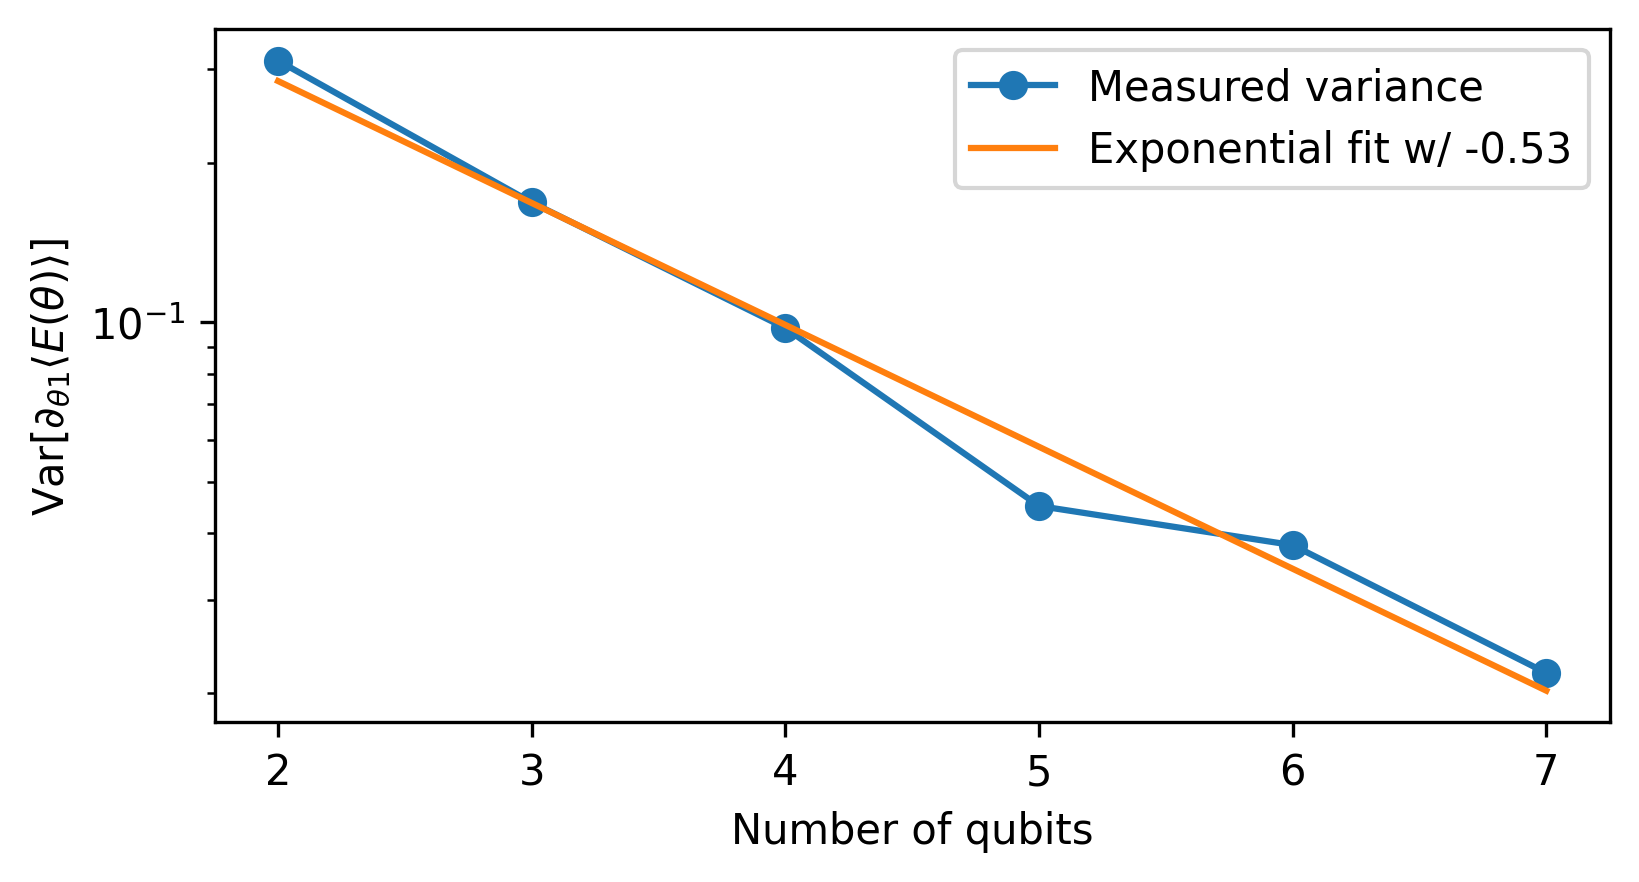
\includegraphics[width=\linewidth]{Artefact/Appendices/var2.png}
        \centerline{2) Layerwise learning}
    \end{subfigure}
    \hfill
    \begin{subfigure}[b]{.49\linewidth}
        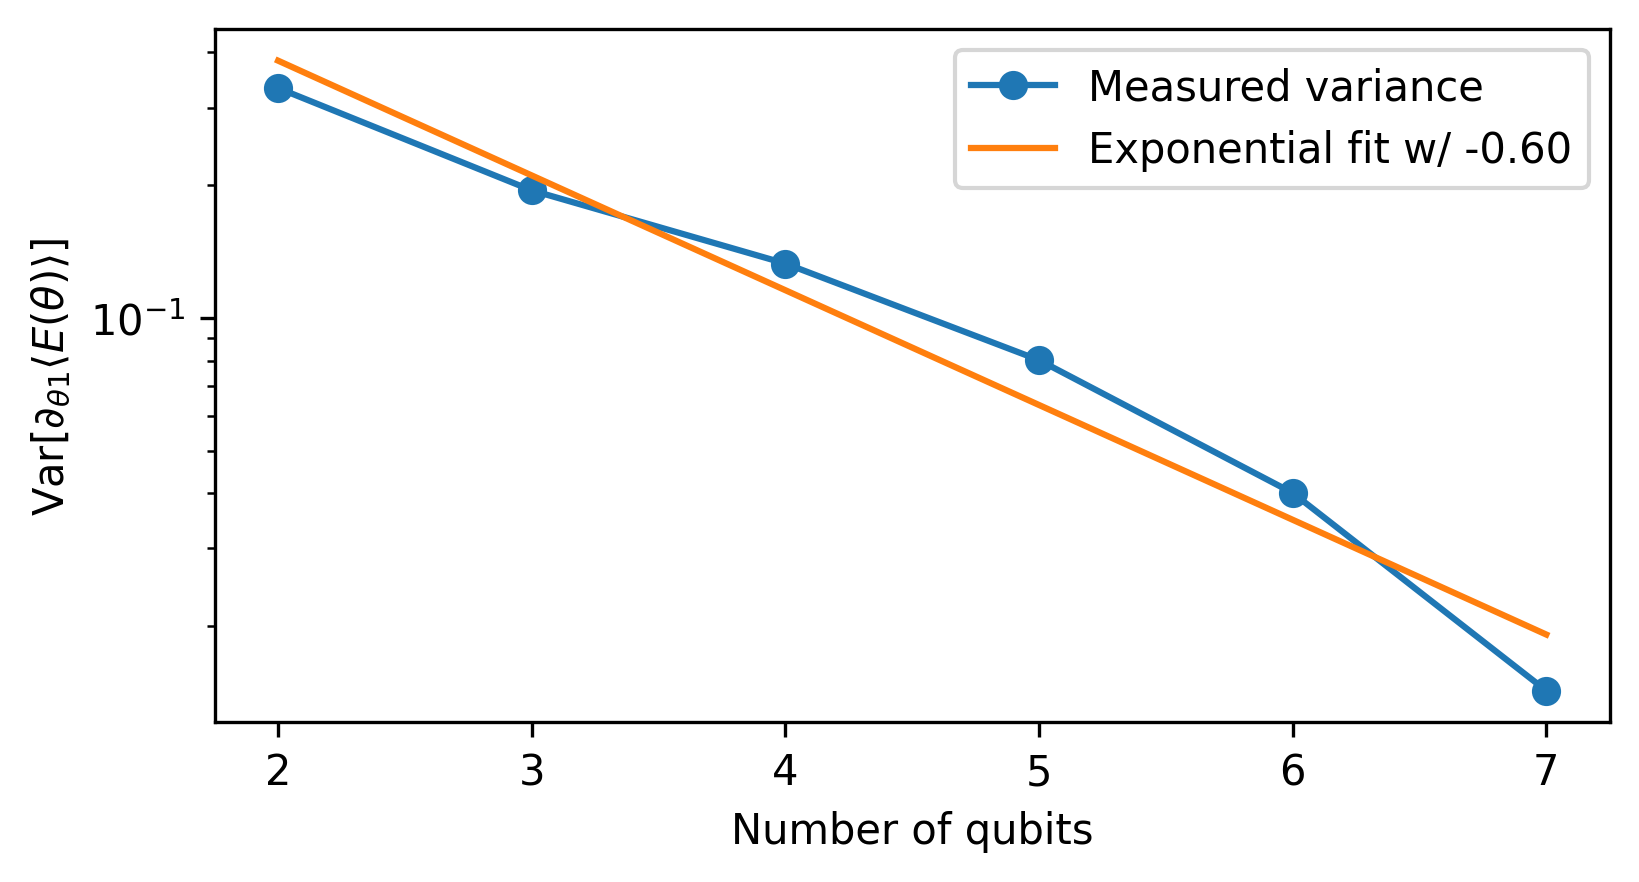
\includegraphics[width=\linewidth]{Artefact/Appendices/var3.png}
        \centerline{3) Identity blocks}
    \end{subfigure}

    \caption{
        The variances of gradient from differences ansatzes in the four configurations.
        For each iteration, we increase the qubit and repetition count by 1, starting from 2 to 7.
        The variances vanish exponentially to the number of qubits.
        For the shallow circuit - local cost function, we keep the repetition value fixed as 1 and only measure two qubits.
    }
    \label{Plot ansatzes variance}
\end{figure}

In contrast, for the case of Local Cost Function and Shallow circuit, we observe that the variances of the ansatz' gradient did not vanish when we attempted to increase the number of qubits.
The slope of the ansatz in this case decay exponentially fit with -0.06.
This implies that the cost function landscape can sustain the slope.
Figure \ref{Plot ansatzes variance}b shows the result of the experiment for local cost function and shallow circuit.
We can see that the ansatz produced an unstable graph which mean the trainability of gradient-based optimization algorithms would not be consistent.
For example, the variance value for 6 qubits is higher compared to 3, 4 or 5 qubits.

To compare the effectiveness of the different treatments, we plot the variance graph of above mention cases in Figure \ref{Fig: Plot Variances} and the Table \ref{Tab: Experiment Phase 1 Res}.
The results have shown the differences in the decay rates of different ansatzes and methods.
Overall, the ansatzes with the local cost function and restriction on circuit depth have their variance values remaining higher and being more consistent for higher qubit count.
The ansatz with this treatment, therefore would not possess a barren plateau.
On the other hand, the values for the other cases shrink exponentially and eventually, the near-zero gradient around the initial point will expand to a large plateau.


\begin{figure}
    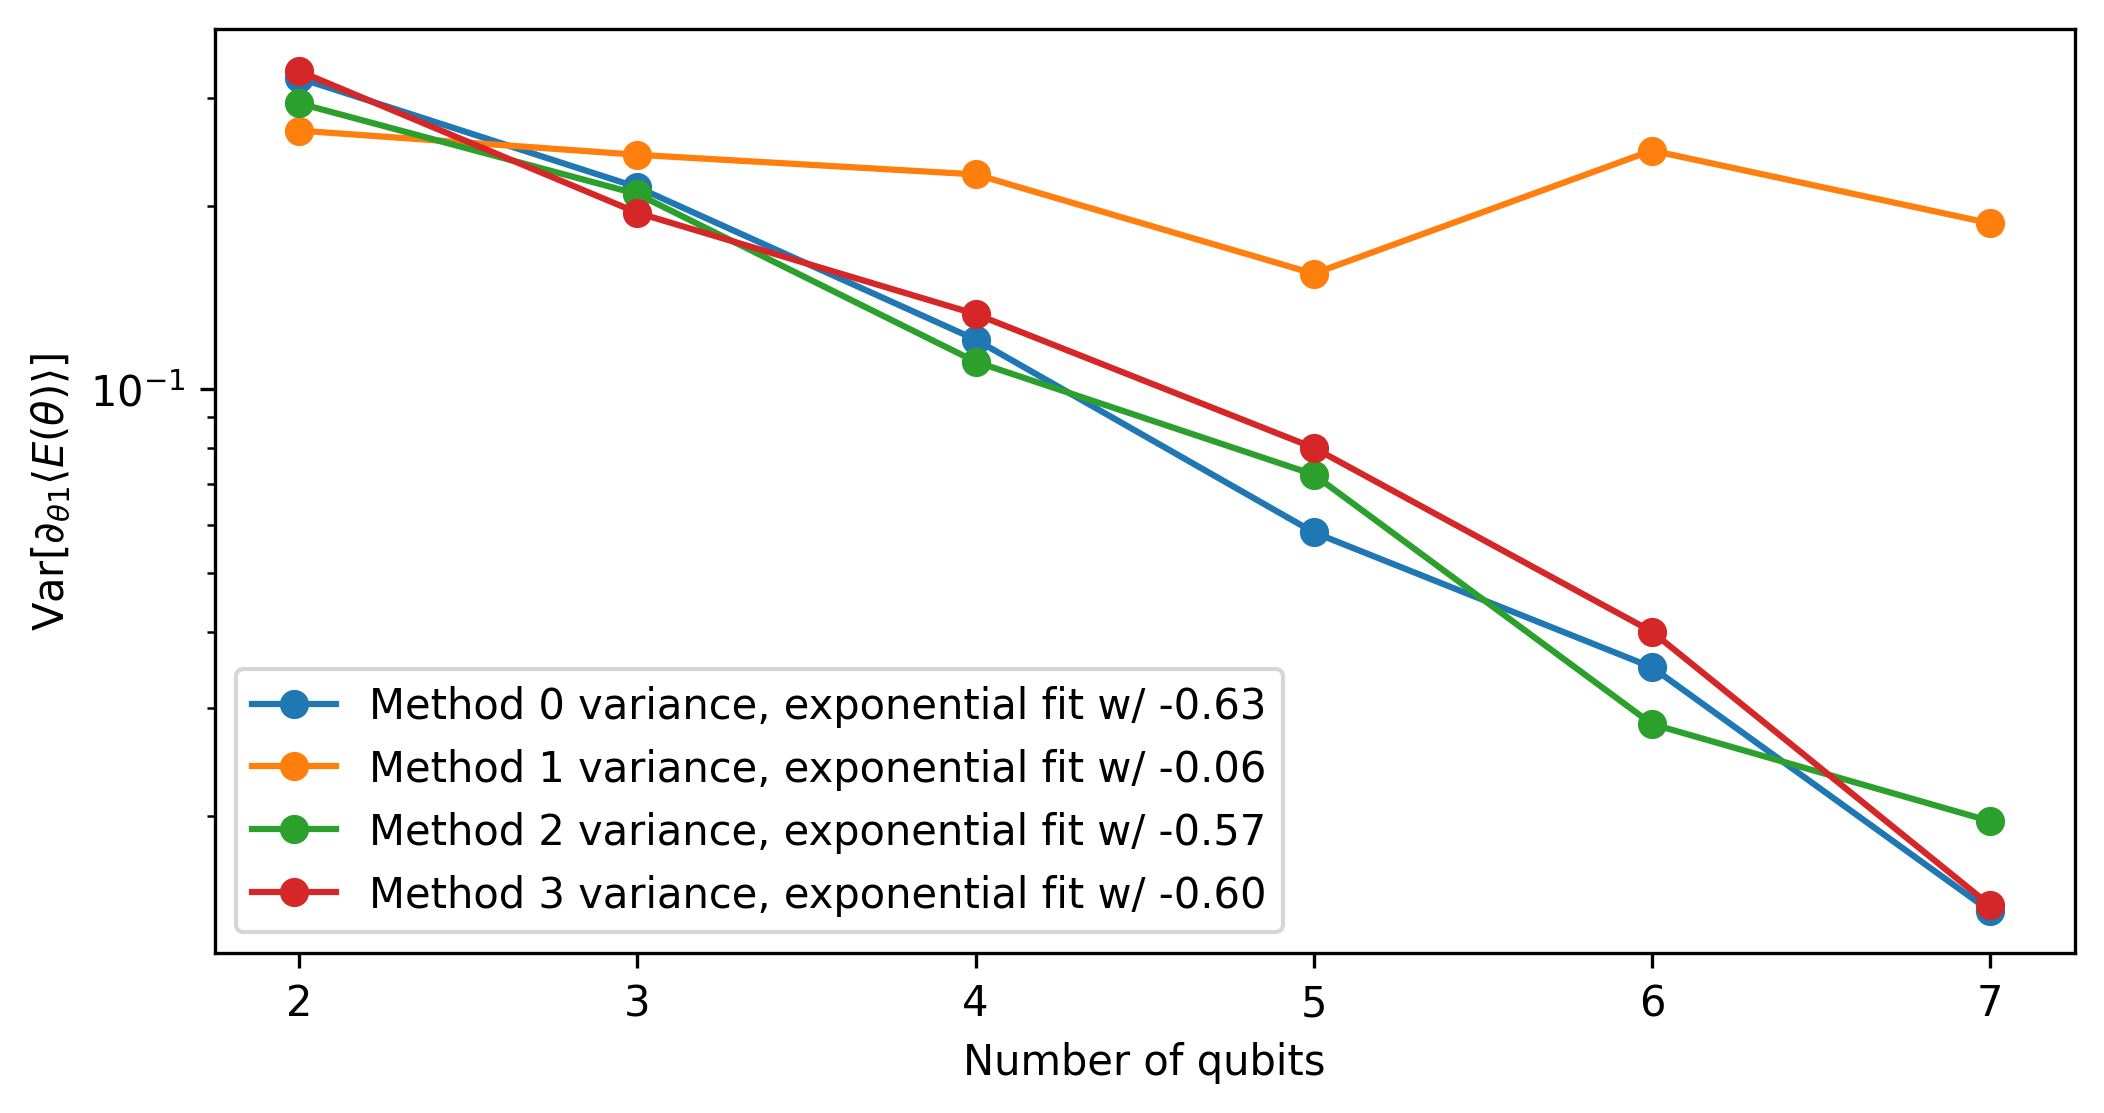
\includegraphics[width=\linewidth]{Artefact/Appendices/variances.png}
    \caption{
        Comparison of the variance values of the ansatzes with four treatments applies.
        The ansatz with local cost function and fixed depth has its variance decay at a significantly smaller rate (-0.06) compared to the rest.
    }
    \label{Fig: Plot Variances}
\end{figure}


\subsubsection{Classification Results}

\begin{table*}
    \centering
    \begin{tabular}{|| p{4cm} p{2cm} p{2cm} p{2cm} p{2cm} ||}
        \hline
        \textbf{Method}                          & \textbf{Circuit depth} & \textbf{Parameters count} & \textbf{Minimum loss} & \textbf{Score} \\
        \hline \hline
        0: No Restriction                        & 15                     & 16                        & 0.57                  & 72.50\%        \\
        1: Local Cost Function - Shallow circuit & 5                      & 6                         & 0.57                  & 80\%           \\
        2: Layerwise Learning                    & 15                     & 16                        & 0.39                  & 92.5\%         \\
        3: Identity Blocks                       & 18                     & 24                        & 0.39                  & 90\%           \\
        \hline
    \end{tabular}
    \caption{
        The result as recorded from the phase two of the experiment.
        We use the ansatzes from four methods as the neural network to solve a classification problem.
    }
    \label{Tab: Experiment Phase 2 Res}
\end{table*}

The unrestricted and local cost function - shallow depth ansatzes loss functions both converged at a value of 0.57.
However, we can see that the local cost function and shallow circuit ansatz achieved higher accuracy in the classification test (at 80\% accuracy) than the unrestricted ansatz (at 72.5\% accuracy).
However, by restricting the ansatz depth, we may have limited the model capacity, this also applies to classical machine learning \cite{ianDeepLearningAdaptive2016}.
As more complex functions would require higher model capacity, thus higher layer count and qubit count, the local cost function - shallow depth method is suitable if the dataset represents a simple function.

\todo{) may have BP, but 1 does not have cap enough to learn, so it converged but still very high}

The identity blocks can achieve a similar loss value as the layerwise learning method (0.39) with a bit lower accuracy.
We can see that with the optimised initial parameters, the loss function can converge faster compared to identity blocks initialisation.
However, it would take more time to obtain the optimal initial parameter due to the training process (see Section \ref{Sec: Method2}), while it is much faster to generate parameters for identity blocks in Section \ref{Sec: Method3}.
The two methods also have their accuracy close to each other, scoring at 92\% for layerwise learning and 90\% for identity blocks.
Thus they are suitable for designing ansatzes of higher layer count to learn more complex functions.


To compare the effectiveness of different approaches, we plot the loss per iteration graph of above mention cases in Figure \ref{Fig: Plot Loss and Accuracy} and Table \ref{Tab: Experiment Phase 2 Res}
Overall, the methods that involve configurations on the initial parameters can achieve lower loss in training and higher score on the classification test.

\begin{figure}
    \begin{subfigure}{\linewidth}
        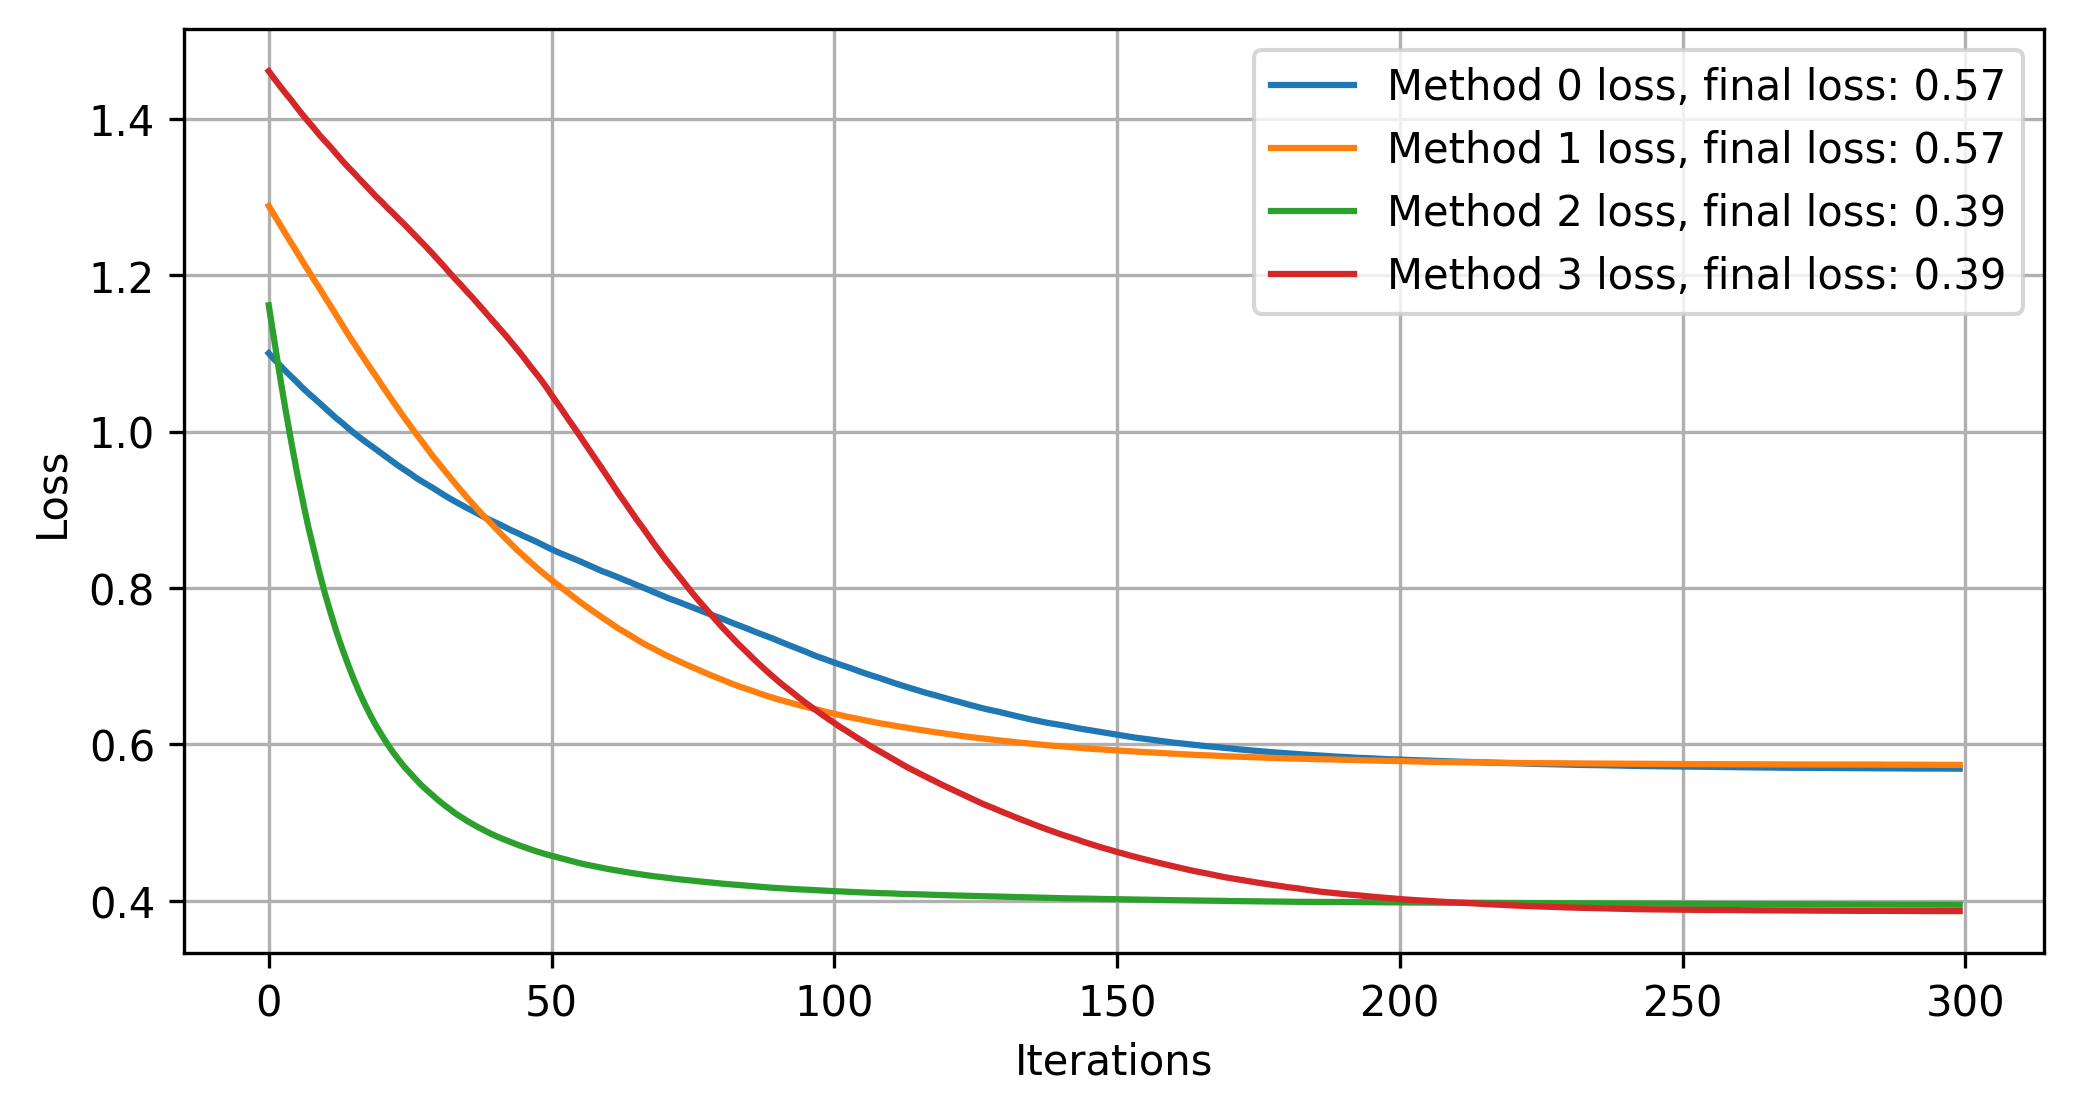
\includegraphics[width=\linewidth]{Artefact/Appendices/loss.png}
        \centerline{a) Loss function values of four classifiers in 300 steps}
    \end{subfigure}
    \begin{subfigure}{\linewidth}
        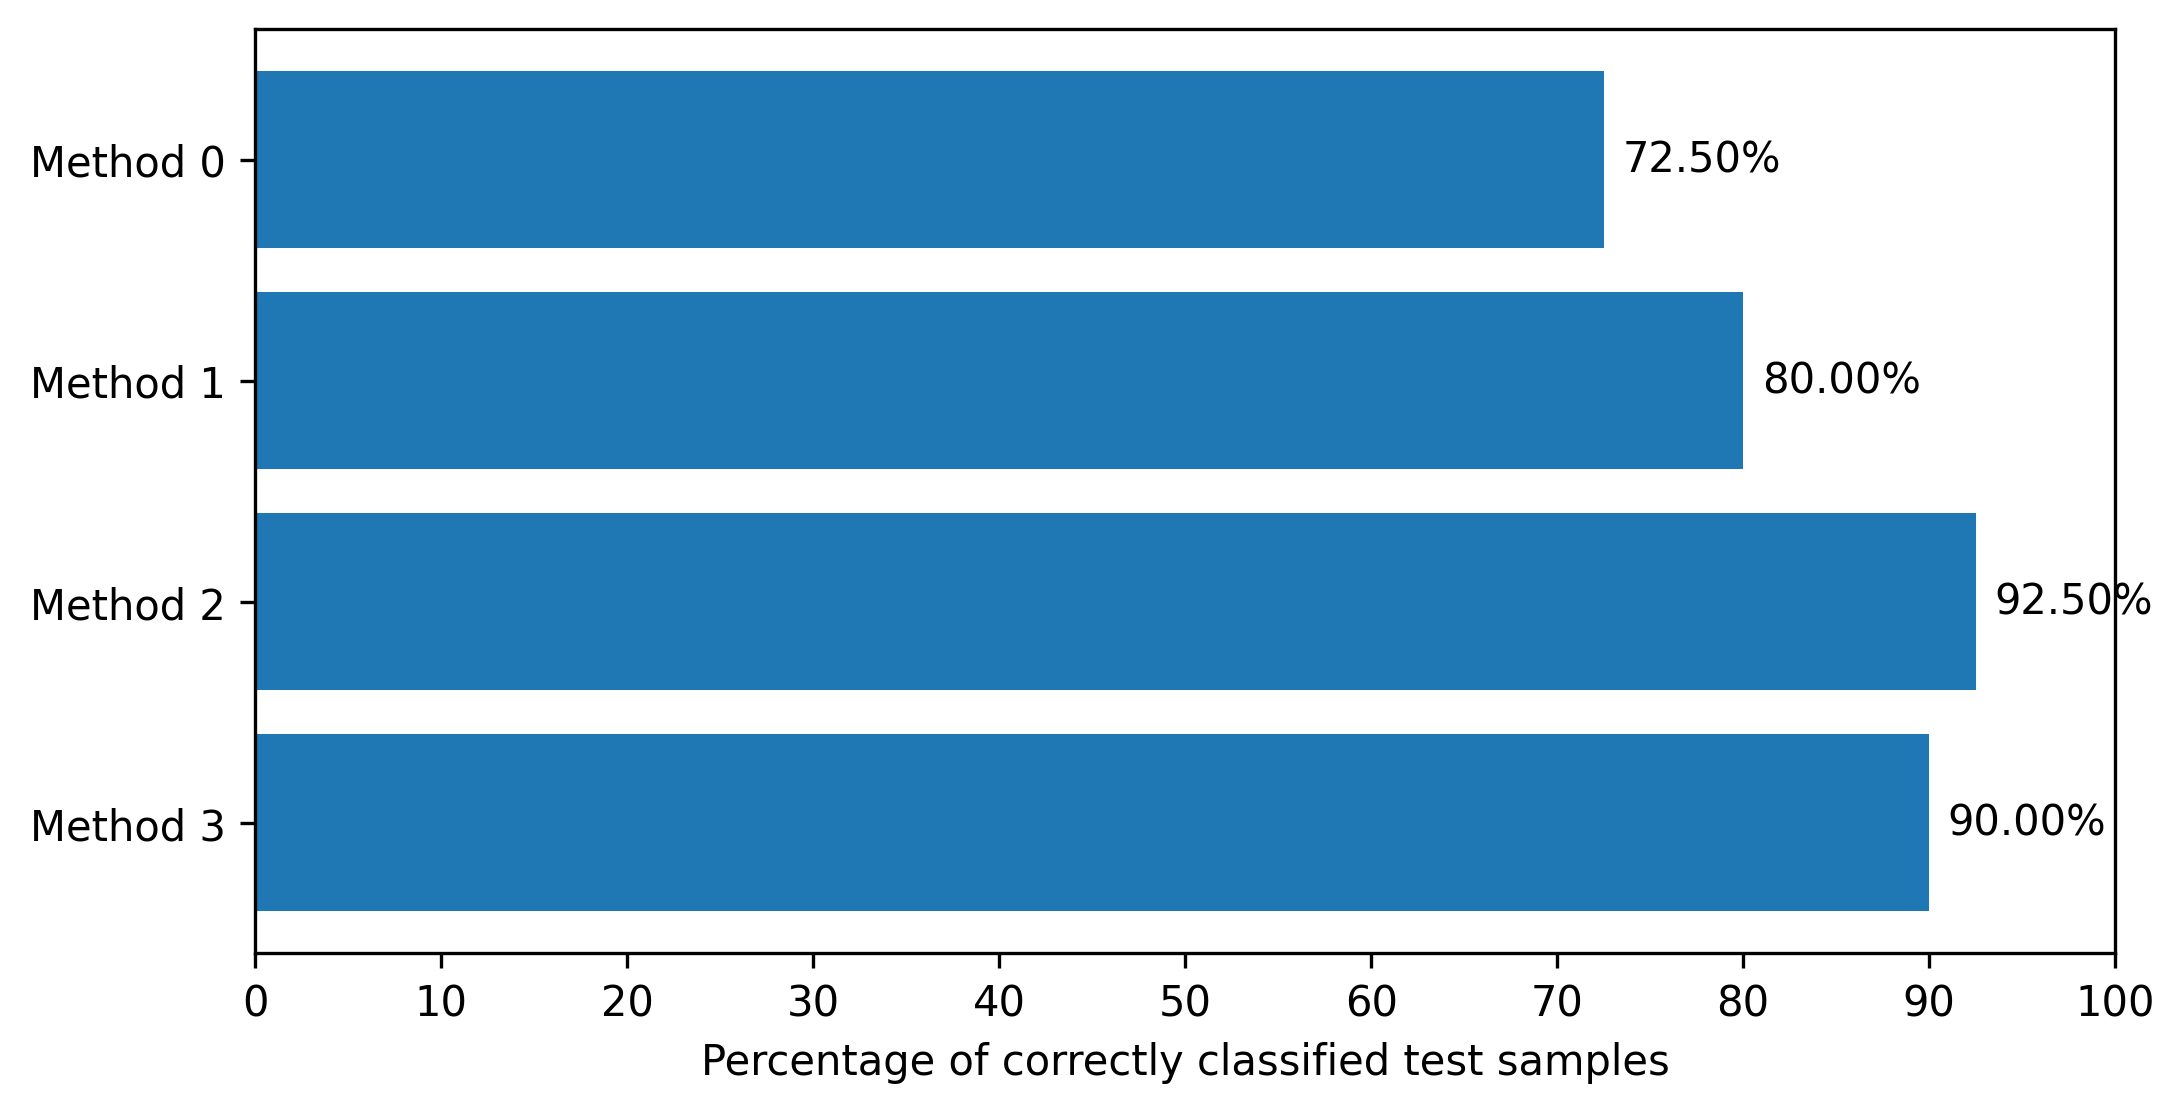
\includegraphics[width=\linewidth]{Artefact/Appendices/accuracy.png}
        \centerline{b) Accuracy score of four classifiers}
    \end{subfigure}

    \caption{
        Comparison of the loss values per iteration of gradient descent for the ansatzes with four treatments applies.
        We measure the accuracy of prediction with a set of 20 testing datapoints.
    }
    \label{Fig: Plot Loss and Accuracy}
\end{figure}


\subsection{Artefact Development Summary}

We have implemented three methods of dealing with barren plateau by altering the ansatz's depth, cost function, and initial parameters aspects.
The experiments have produced the results as the slopes of the gradients for a number of qubits, as well as the performance of ansatzes in neural network training.
The results indicate that the variances of the gradient can be stable if we set a limit on the length of the circuit and the cost function, and the training performance can increase if we carefully select the initial parameters.

With this artefact, we have addressed the research design in Section \ref{Research Design section}.
We have implemented the three methods, namely \textit{local cost function, shallow ansatz depth}, \textit{layerwise learning} and \textit{identity blocks}.
We have compared the variances in the first phase of the experiment.
We anticipate that a higher variance value does not mean the optimisation is going in the right direction, the model can still stick it in a local minimum, or the error landscape is random.
To verify the performance of these methods, in the second phase, we implemented a variational quantum neural network to solve a classification problem with a standard dataset.

The phase two of the experiments have verified that the unrestricted configuration may have run into a barren plateau, while the others can converge to their minimums - the answers.
Moreover, these experiments are conducted in an emulated environment with a noise model from \emph{ibm\_perth} backend.
Thus, this experiment can reflect the real-life situation to some extent.

According to Figure \ref{Fig: Plot Variances}, the variance values of the limited depth - cost function method at seven qubits configuration is significantly higher than the rest.
At higher qubit configuration, the barren plateaus are also more likely to appear, and the performance of these methods under this phenomenon is worth investigating.

